\begin{wrapfigure}{l}{0pt}
  \centering
  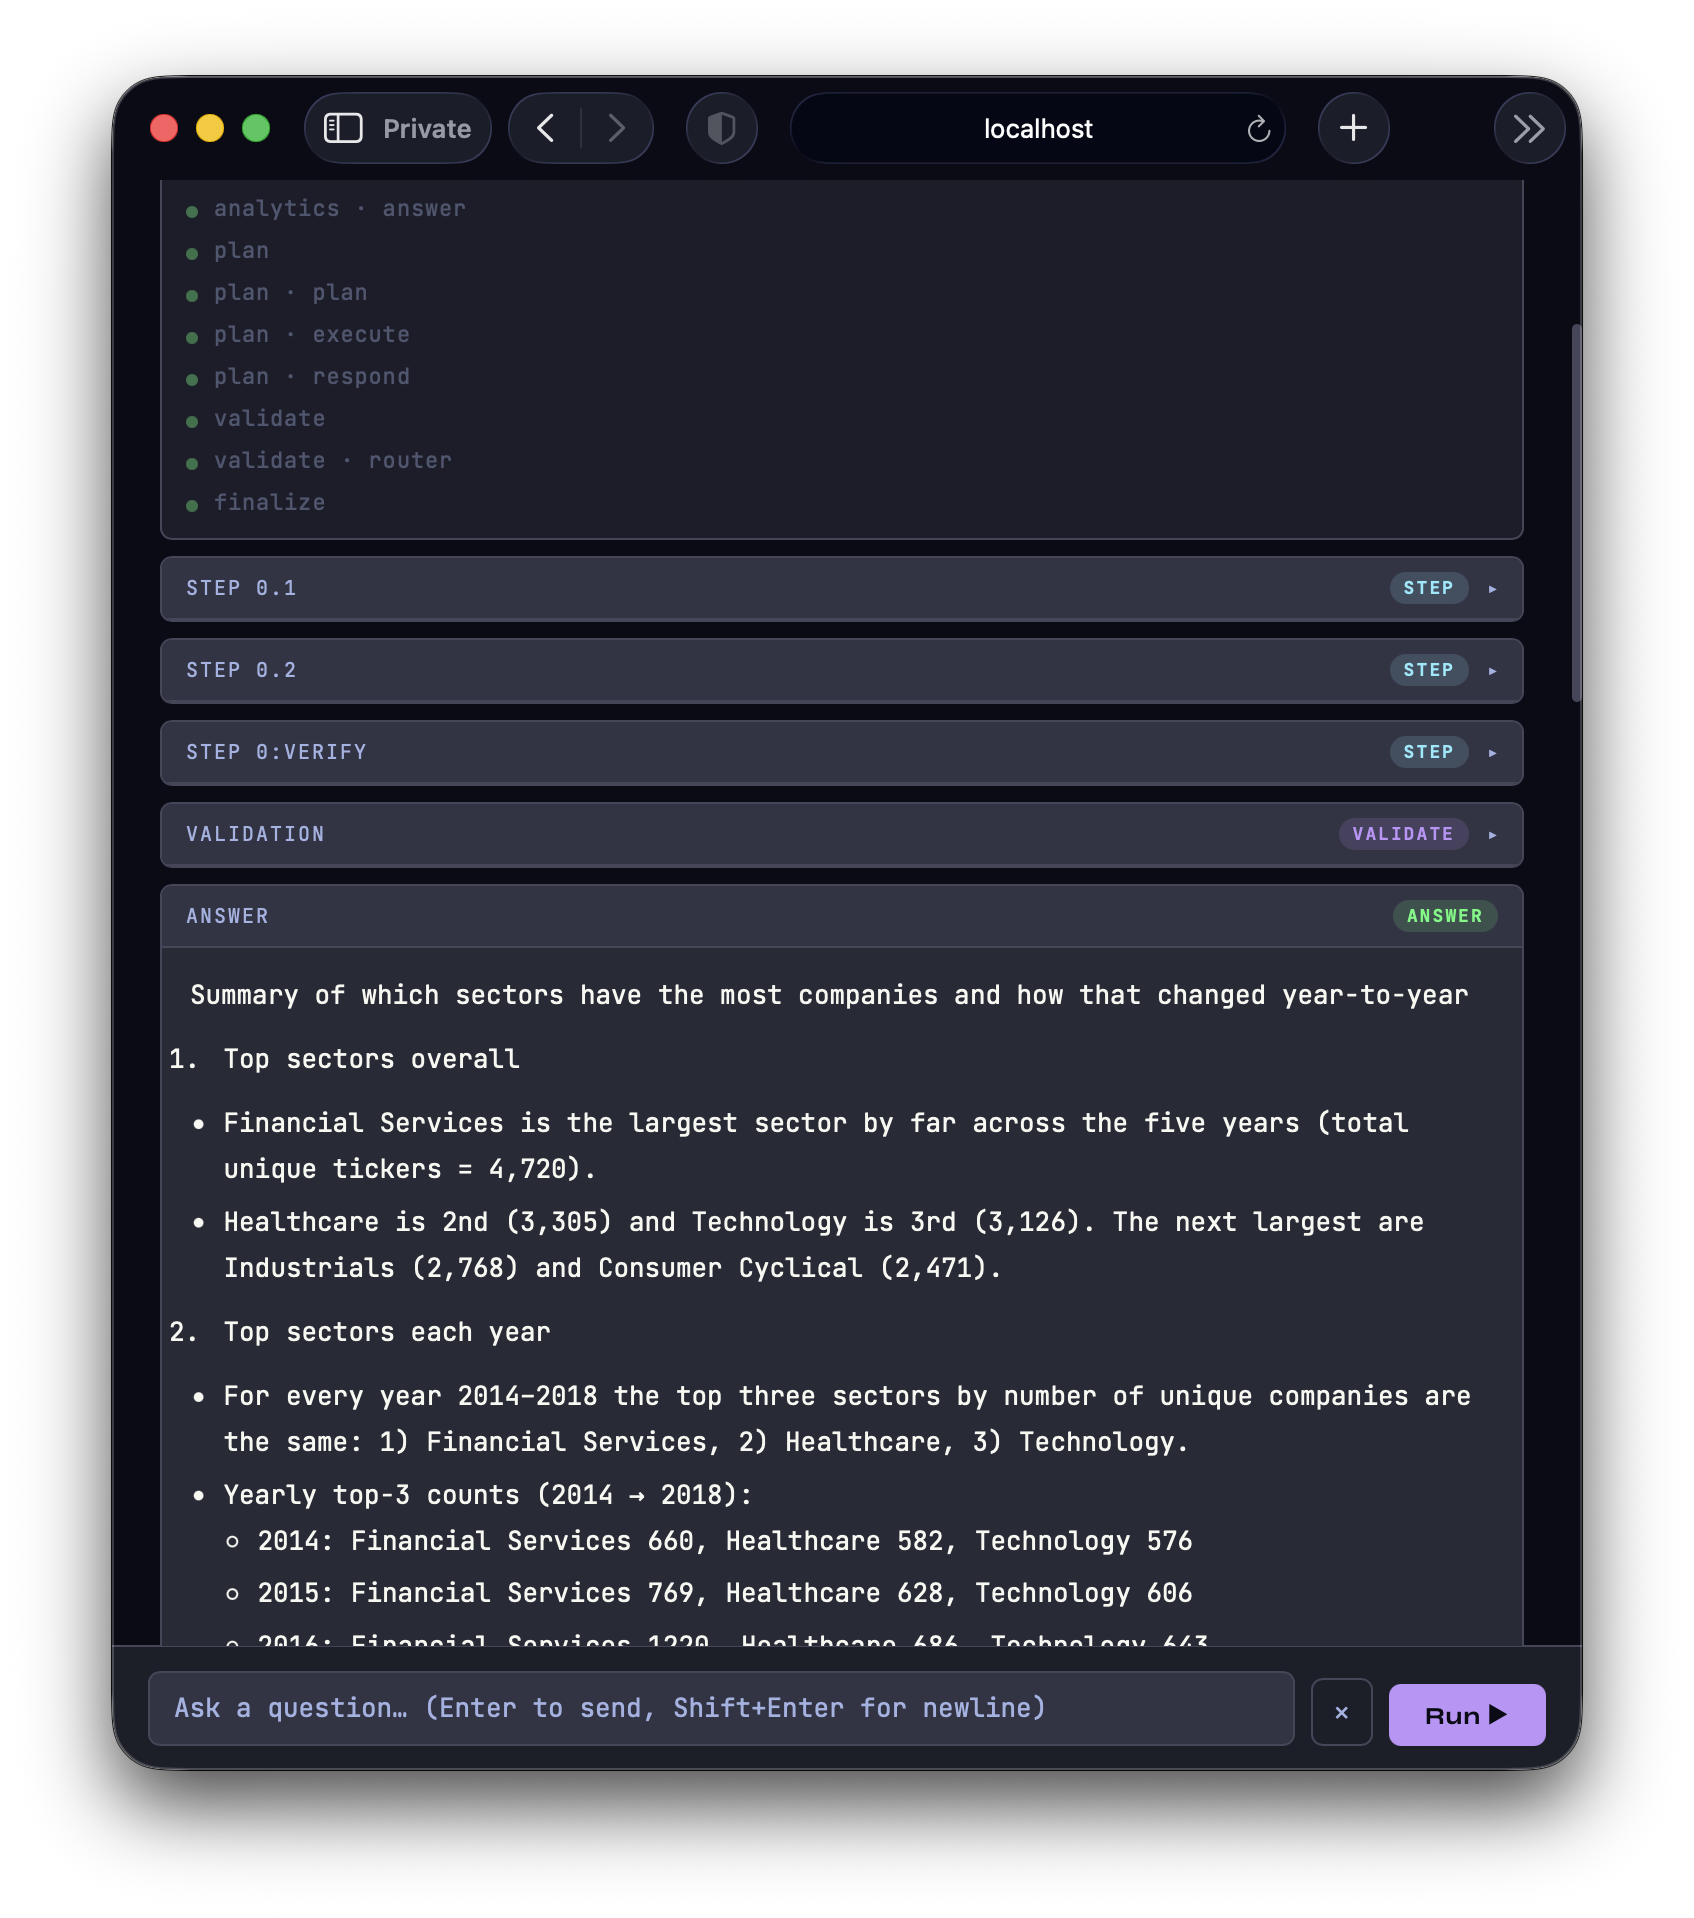
\includegraphics[width=0.4\textwidth]{graphics/ui-which-sectors-have-the-most-companies-represented,-and-how-does-that-distribution-change-year-to-year.png}
  \caption{UI Screenshot}
\end{wrapfigure}

The agent followed a multi-stage analytical workflow. The process combined data aggregation, normalization, ranking, visualization, and interpretation steps before producing the final summary.

\subsect{Understanding the Analytical Objective}

The agent first translated the natural-language question into a quantitative task. It identified that the goal was not simply to count records, but to determine how many distinct companies were represented within each sector for every year. Because companies could appear multiple times within a dataset, the agent chose to count unique ticker symbols rather than raw rows.

The agent also recognized that answering the second part of the question required comparing sector distributions across years, which necessitated both absolute counts and normalized percentages.

\subsect{Extracting Year Information and Preparing Annual Statistics}

The agent processed each yearly financial dataset independently. For every file, it extracted the year from the filename and grouped observations by sector.

Within each sector, the agent computed the number of unique ticker symbols using a distinct-count aggregation. This produced a sector-level company count for each year from 2014 through 2018.

This step transformed the raw company-level datasets into a compact representation that captured the number of companies operating within each sector during each year.

\subsect{Combining Yearly Results into a Unified Table}

After computing annual sector counts, the agent merged the results into a single table with:

\begin{itemize}
  \item sectors as rows,
  \item years as columns, and
  \item unique-company counts as values.
\end{itemize}

Missing sector--year combinations were filled with zeros to ensure consistency across all years. The resulting matrix enabled direct comparison of sector representation over time.

The agent also calculated total company counts across all years for each sector and sorted sectors by these totals. This ranking made it easier to identify the most heavily represented sectors overall.

\subsect{Normalizing Counts to Measure Distribution Changes}

The agent recognized that absolute company counts alone would not fully describe how sector representation changed over time. To measure relative representation, it normalized the counts within each year.

Specifically, the agent divided each sector's count by the total number of companies in that year, producing percentage shares. These percentages allowed the agent to compare sector composition across years even when the total number of companies varied between datasets.

This normalization step was essential for identifying whether changes reflected genuine shifts in sector representation rather than differences in dataset size.

\subsect{Generating Visual Summaries}

\begin{wrapfigure}{l}{0pt}
  \centering
  \includegraphics[width=0.4\textwidth]{report-data/which-sectors-have-the-most-companies-represented,-and-how-does-that-distribution-change-year-to-year/plot-sector-distribution-by-year-stacked.png}
  % \caption{UI Screenshot}
\end{wrapfigure}

To support interpretation, the agent created two visualizations.

First, it produced a stacked bar chart showing sector composition for each year. This visualization highlighted how the overall distribution of companies was allocated among sectors and how those allocations evolved over time.

\begin{wrapfigure}{r}{0pt}
  \centering
  \includegraphics[width=0.4\textwidth]{report-data/which-sectors-have-the-most-companies-represented,-and-how-does-that-distribution-change-year-to-year/plot-top-6-sector-trends.png}
  % \caption{UI Screenshot}
\end{wrapfigure}

Second, it generated a line chart tracking the largest sectors across years. By focusing on the most represented sectors, the chart emphasized long-term trends and made year-to-year changes easier to observe.

These visual outputs complemented the numerical tables and provided a clearer view of temporal patterns.

\subsect{Identifying Dominant Sectors and Yearly Leaders}

With the aggregated data available, the agent examined sector rankings both overall and within individual years.

It computed total company counts across the entire period to determine the most represented sectors overall. It also identified the top sectors within each year by sorting annual counts and extracting the leading categories.

This analysis revealed whether sector leadership changed over time and whether any sectors consistently dominated the dataset.

\subsect{Analyzing Temporal Trends}

The agent then compared both counts and percentage shares across years to identify notable trends.

Rather than merely reporting rankings, it examined how sector representation evolved over time. Particular attention was given to sectors exhibiting unusually large increases or decreases, since these changes were most relevant to the question of distributional change.

The agent compared annual percentages, assessed stability versus volatility among sectors, and highlighted sectors whose representation shifted substantially relative to others.

\subsect{Producing the Final Interpretation}

After completing the quantitative analysis, the agent synthesized the results into a concise narrative. The final response summarized:

\begin{itemize}
  \item the sectors with the largest overall representation,
  \item the leading sectors in each year,
  \item changes in sector shares over time,
  \item notable increases and decreases in representation, and
  \item the broader trends revealed by the visualizations.
\end{itemize}

The final answer therefore emerged from a sequence of reasoning stages: data preparation, unique-company aggregation, cross-year integration, normalization, visualization, ranking, trend analysis, and narrative interpretation.
